\section{証明}
\label{section:differentiable}

本節では次の手順で定理\ref{DifferentiableIsPspace}, \ref{KTimesIsCH}を示す. 
まずある種の差分方程式の族が, 
$\classPSPACE$困難ないし$\classCH$困難であることを示す
(\ref{section:divp}節, \ref{subsection: counting hierarchy}節).
そしてこの差分方程式が, 
滑らかさの条件を満たす\eqref{eq:ode}の形の微分方程式の族により模倣されることを示す
(\ref{subsection: ode family}節). 
この族を一つの滑らかな微分方程式へ埋め込むことで, 
定理にいう$g$, $h$を構成する(\ref{subsection: proof of theorems}節).

このように微分方程式で差分方程式を模倣する考え方は, 
既にLipschitz条件の場合の証明
\cite{kawamura2010lipschitz}にも本質的には現れていたものであるが, 
本稿ではより精密に, 滑らかさの条件が与える影響を調べるため, 
差分方程式の構造に着目する. 
その結果, 
$2$回以上連続微分可能という制限の下でも, 
差分方程式族の「深さ」が小さければ模倣できることが判り, 
そのことから$\classCH$困難性が従う. 

\subsection{差分方程式}
\label{section:divp}

この節では微分方程式\eqref{eq:ode}の離散版ともいうべき差分方程式を定義し, 
それが深さの制限に応じて
$\classPSPACE$困難ないし$\classCH$困難であることを示す.

$[n] = \{0, \dots , n-1\}$と書く.
関数$G \colon [P] \times [Q] \times [R] \to \{-1, 0, 1\}$と
$H \colon [P + 1] \times [Q+1] \to [R]$が
任意の$i \in [P]$, $T \in [Q]$について以下を満たすとき(図\ref{fig:divp}), 
\begin{figure}
 \begin{center}
  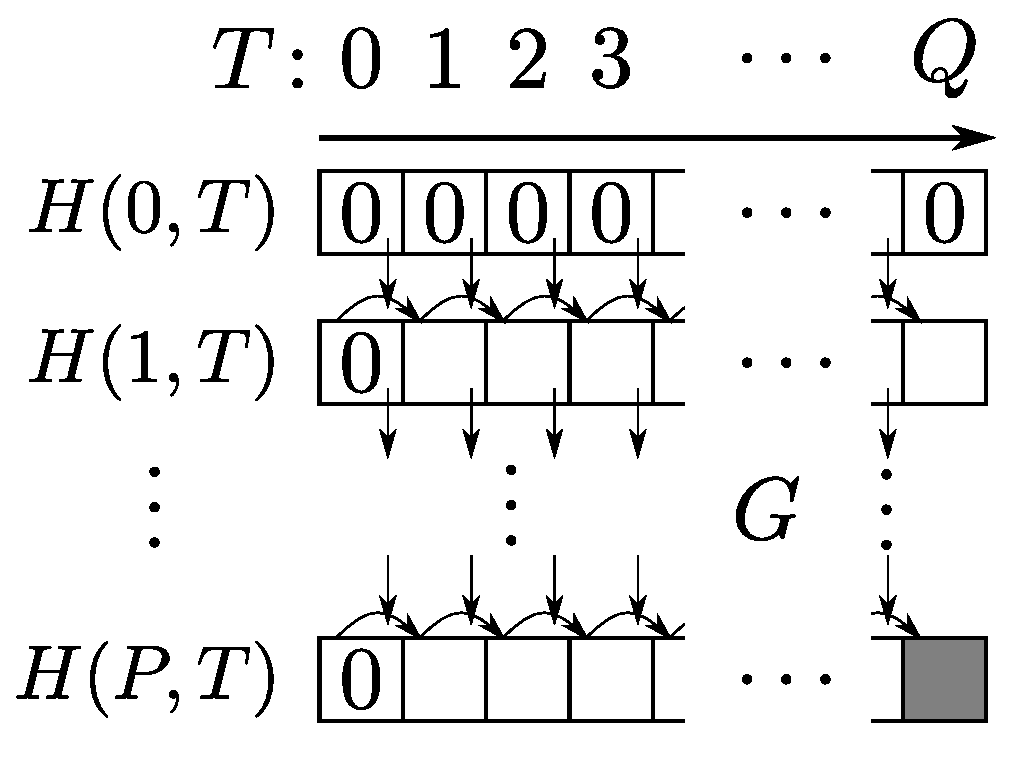
\includegraphics[height=0.15\textheight]{image/divp.eps}
 \end{center}
 \caption{差分方程式$G$とその解$H$}
 \label{fig:divp}
\end{figure}
$H$を\emph{差分方程式}\kern\xkanjiskip$G$の解と呼ぶ.
\begin{gather}
   H(i, 0) = H(0, T) = 0 \label{eq:initial value}
\\
   H(i + 1, T + 1) - H(i+1, T) = G(i, T, H(i, T))  \label{eq:divp}
\end{gather}
$P$, $Q$, $R$をそれぞれこの差分方程式の
\emph{段数}, \emph{列数}, \emph{欄の大きさ}と呼ぶ.
\eqref{eq:ode}の初期条件$h(0) = 0$と方程式$\D h(t) = g(t, h(t))$が
それぞれ式\eqref{eq:initial value}, \eqref{eq:divp}に似ており, 
\ref{subsection: ode family}節ではこれを用いて
微分方程式で差分方程式を模倣する. 


文字列$u$ごとに一つの差分方程式$G _u$を与え,
$u$が言語$L$に属するかをその差分方程式によって計算することを考える.
各 $u$ に対して $G_u$ の段数と列数, 解をそれぞれ $P_u, Q_u, H_u$ としたとき,
言語$L$が関数族$(G_u)_u$によって
\emph{認識}されるとは,
$H_u(P_u, Q_u) = L(u)$ を満たすこととする.

族$(G_u)_u$が\emph{一様}であるとは,
$G_u$の段数, 列数, 欄の大きさそれぞれを$u$を入力とする関数と見做したとき
それらが多項式時間計算可能であり,
かつ与えられた$(u, i, T, Y)$から多項式時間で$G_u(i, T, Y)$が
計算できることと定義する.
そのようなとき$G _u$の段数, 列数及び欄の大きさは,
$|u|$の多項式の指数($2^{\mathrm{poly} (|u|)}$)で抑えられる.
$G_u$の段数を$P_u$と置くとき, 多項式$p$が存在して$P_u \le p(|u|)$が成立つとき,
族 $(G_u) _u$は\emph{多項式段}であるという.
また定数$c,d$が存在して$P_u \le c \log(|u|)+d$が成立つとき,
族 $(G_u) _u$は\emph{対数段}であるという. 
この用語を使うと, 
河村がLipschitz連続な場合の解析に用いた補題
\cite[補題4.7]{kawamura2010lipschitz}は次のように書ける. 

\begin{lemma}
 \label{DIVPpolyIsPSPACEhard}
 多項式段の一様な差分方程式族によって認識される$\classPSPACE$困難な言語が存在する
 \footnote{差分方程式によって認識される言語のクラスはカープ帰着において閉じており,
多項式段一様な関数族によって認識される言語は$\classPSPACE$と一致する.}.
\end{lemma}

河村\cite{kawamura2010lipschitz}は
この多項式段の一様な差分方程式族をLipschitz連続な微分方程式で模倣することで, 
表\ref{table:related}第三行の結果を得た. 
本稿の定理\ref{DifferentiableIsPspace}はこの構成に手を加えて, 
$(\infty, 1)$回微分可能な模倣に
作り替えることにより
(\ref{subsection: ode family}, \ref{subsection: proof of theorems}節), 
やはり補題\ref{DIVPpolyIsPSPACEhard}から得られる. 

本稿では更に, 対象とする差分方程式族を対数段に制限すれば, 
$(\infty, 2)$回以上微分可能な関数によっても
模倣できることを示し
(\ref{subsection: ode family}, \ref{subsection: proof of theorems}節), 
これと次の補題から定理\ref{KTimesIsCH}を得る. 

\begin{lemma}
 \label{DIVPlogIsCHhard}
 対数段の一様な差分方程式族によって認識される$\classCH$困難な言語が存在する.
\end{lemma}

計数階層$\classCH$の定義と差分方程式の関係及び
補題\ref{DIVPlogIsCHhard}の証明は
\ref{subsection: counting hierarchy}節にて述べる.


\subsection{計数階層と対数段の差分方程式}
\label{subsection: counting hierarchy}

\emph{計数階層}\kern\xkanjiskip(Counting Hierarchy) $\classCH$は
Wagnerによって導入された計算量クラスである\cite{wagner1986complexity}.
多項式階層$\classPH$が$\classNP$の神託機械を用いて
\begin{align}
 \classSigma^p_0  &= \classP
 &
 \classSigma^p_{n+1} &= \classNP ^{\classSigma^p_n}
 &
 \classPH &= \bigcup_n \classSigma^p_n
\end{align}
と定義されるのに対し,
計数階層は多項式階層の$\classNP$を$\classPP$で置き換えて
\begin{align} \label{eq:CH}
 \quantC_0 \classP  &= \classP
 &
 \quantC_{n+1} \classP &= \classPP^{\quantC_n \classP}
 &
 \classCH &= \bigcup_n \quantC_n \classP
\end{align}
で定義される\footnote{ただしこの特徴づけは Tor{\'a}n によるものであり,
Wagnerによる定義とは異なる\cite{toran1991complexity}.
}. $\classPH \subseteq \classCH \subseteq \classPSPACE$だが,
いずれも真の包含か否かは未解決である.



各階層$\quantC_n \classP$は次の完全問題$\quantC_n B_{be}$をもつ.
量化子 $\quantC$ を自然数 $m$, $l$ 個の論理変数の組 $X$,
論理式$\phi(X)$について次のように定義する.
\begin{equation}
 \quantC^m X \phi(X) 
  \longleftrightarrow 
  \sum_{X \in \{0,1\}^l} \phi(X) \ge m.
\end{equation}
ただし論理式$\phi(X)$を関数$\phi \colon \{0,1\}^l \to \{0,1\}$と同一視し,
$\phi(X)$が成立つとき$\phi(X)=1$とする.
$\quantC^1 = \exists$, $\quantC^{2^l} = \forall$ であり, $\quantC$ は $\exists, \forall$ の
一般化と言える.
言語$\quantC_n B_{be}$を次のように定義する.
\begin{equation}
 \langle \phi(X_1, \dots, X_n), m_1, \dots, m_n \rangle \in \quantC_n B_{be}
 \longleftrightarrow
 \quantC^{m_1}{X_1} \cdots \quantC^{m_n}{X_n} \phi(X_1, \dots, X_n) 
\end{equation}
ただし
$X_i$ は論理変数の組,
$\phi(X_1, \dots, X_n)$は$X_1, \dots, X_n$以外の変数を持たない論理式とする.

\begin{lemma}[{\cite[定理7]{wagner1986complexity}}] \label{lemma:CnP-complete}
 $\quantC_n B_{be}$ は $\quantC_n\classP$ 完全.
\end{lemma}

これらの問題$\quantC_n B_{be}$から問題$\quantC_{\log} B_{be}$を次で定義する.
\begin{equation}
 \langle 0^{2^n}, u \rangle \in \quantC_{\log} B_{be}
 \longleftrightarrow
 u \in \quantC_n B_{be}
\end{equation}
この$\quantC_{\log} B_{be}$が補題\ref{DIVPlogIsCHhard}で求める言語であること,
つまり$\classCH$困難かつ対数段一様関数族によって認識可能であることを示す.

\begin{proof}[\textup{補題\ref{DIVPlogIsCHhard}の証明}]
 $\quantC_{\log} B_{be}$が$\classCH$困難であることを示す.
 任意の $\classCH$ の言語 $A$ はある階層 $\quantC_n \classP$ に属する. 
 補題 \ref{lemma:CnP-complete} より任意の $u \in \{0,1\}^*$ について
 $u \in A \leftrightarrow f_n(u) \in \quantC_n B_{be}$ 
 を満たす多項式時間関数 $f_n$ が存在する.
 \begin{align}
  u \in A 
  & \longleftrightarrow \langle 0^{2^n}, f_n(u) \rangle \in \quantC_{\log} B_{be}
 \end{align}
 $n$ は定数であるため $\langle 0^{2^n}, f_n(\cdot) \rangle$ は多項式時間関数.
 よって $A$ は $\quantC_{\log} B_{be}$ に帰着する.


 $\quantC_{\log} B_{be}$を認識する対数段一様な関数族 $(G_u)_u$ を構成する.
 自然数 $n, m_1, \dots, m_n$, 論理式$\phi$を
 $u  = \langle 0^{2^n}, 
 \langle \phi(X_1, \dots, X_n), m_1, \dots, m_n \rangle \rangle$
 を満たすものとする. 
 (そのような$n, m_1, \dots, m_n, \phi$が存在しないとき$u \not \in A$.)
 
 
 $l_i = |X_i|$, $s_i = i + \sum^i_{j=1}l_j$ と表記する.
 任意の $i \in \{0, \dots, n\}$ と $n-i$ 個の文字列 
 $Y_{i+1} \in \{0,1\}^{l_{i+1}}, \dots, Y_n \in \{0,1\}^{l_n}$ 
 について論理式
 $\quantC^{m_{i}}{X_i} \cdots \quantC^{m_1}{X_1}
 \phi(X_1, \dots, X_i, Y_{i+1}, \dots, Y_n)$
 の真偽値を $\phi_i(Y_{i+1}, \dots, Y_n)$ と表記すると,
 $\phi_0 = \phi$ かつ $\phi_n() = \quantC_{\log} B_{be} (u)$.
 関数 $C^m \colon \N \to \N$ を
 \begin{equation}
  C^m(x) 
     = \begin{cases}
       1 & (x \ge m) \\
       0 & (x < m) 
       \end{cases}
 \end{equation}
 と定義すると
 \begin{equation} \label{eq:phi-step}
  \phi_{i+1}(Y_{i+2}, \dots, Y_n) 
  = C^{m_{i+1}}\left(\sum_{X_{i+1} \in \{ 0,1 \} ^{l_i}}
   \phi_i(X_{i+1}, Y_{i+2}, \dots, Y_{n})\right) 
 \end{equation}
 $T \in \N$ に対し, $T_i$ を $T$ の2進表記における $i$ 桁目, 
 $T_{[i,j]} = T_{j-1} T_{j-2} \cdots T_{i+1} T_{i}$ と表記する.


 $G_u$ を $(i, T, Y) \in [n+1] \times [2^{s_n}+1] \times [2^{|u|}]$ の範囲で
 を以下のように定義する. 一段目つまり $i=0$ ならば
 \begin{equation}\label{eq:def-Gu:case0}
  G_u(0,T,Y) = 
   (-1)^{T_{s_1}}\phi(T_{[1,s_1]}, T_{[s_1+1,s_2]},
    \dots, T_{[s_{n-1}+1,s_n]}) 
 \end{equation}
 $i \ge 1$ ならば
 \begin{equation} 
  G_u(i,T,Y) = 
   \begin{cases}
    (-1)^{T_{s_{i+1}}} C^{m_i}(Y) 
    & (T_{[1,s_i+1]} = 10 \cdots 0) \\
    0 & (\text{othewise}).
   \end{cases} 
 \end{equation}

 差分方程式$G_u$の解を$H_u$と表記する.
 任意の $i \in [n+1]$, $T \in [2^{s_n}+1]$ について,
 $T_{[1, s_i +1]} = 10 \cdots 0$ ならば
 \begin{equation} \label{eq:subformula}
  G_u(i,T,H_u(i,T)) = (-1)^{T_{s_{i+1}}} 
   \phi_i(T_{[s_i+1, s_{i+1}]}, \dots, T_{[s_{n-1}+1, s_n]})
 \end{equation}
 を満たすことを $i$ についての帰納法により示す.

 $i=0$のとき, 式\eqref{eq:def-Gu:case0}より成立つ.
 $i=j$において成立つと仮定すると, 
\begin{equation}
  H_u(j+1, T) 
  = \sum_{V = 0}^{T-1} G_u(j, V, H_u(j, V)) 
  = \sum_{V} (-1)^{V_{s_{j+1}}} \phi_j(V_{[s_j+1, s_{j+1}]}, 
   \dots, V_{[s_{n-1}+1, s_n]})
\end{equation}
 $U \in \{0,1\}^*$に対して, $U$を2進数と解釈した時の値を$\overline U$と表記する.
 $V \le \overline{T_{[s_{j+1}+1, s_n]} 0 \cdots 0}$ の範囲においては
 $\phi_j(V_{[s_j+1, s_{j+1}]}, \dots, V_{[s_{n-1}+1, s_n]})$ と
 $- \phi_j(V_{[s_j+1, s_{j+1}]}, \dots, V_{[s_{n-1}+1, s_n]})$が互いに打ち消し合うので, $T_{[1,s_{j+1} +1]} = 10 \cdots 0$ により,
 \begin{equation}
  H_u(j+1, T) = \sum_{X \in \{0,1\}^{l_j}}
  \phi_j(X, T_{[s_{j+1}+1, s_{j+2}]}, \dots, T_{[s_{n-1}+1, s_n]})
 \end{equation}
 式\eqref{eq:phi-step}より
 \begin{align}
  G_u(j+1,T,H_u(j+1,T)) 
  &= (-1)^{T_{s_{j+2}}} C^{m_{j+1}} (H_u(j+1, T))
\notag
\\
  &= (-1)^{T_{s_{j+2}}} \phi_{j+1}(T_{[s_{j+1}+1, s_{j+2}]}, \dots, T_{[s_{n-1}+1, s_n]})
 \end{align}
 $i=j+1$でも成立つため, 任意の$i \in [n+1]$で\eqref{eq:subformula}が成立つ.


 \eqref{eq:subformula}に $i=n$, $T=2^{s_n}$ を代入して 
 $G_u(n, 2^{s_n}, H_u(n,2^{s_n})) = \phi_n() = \quantC_{\log} B_{be}(u)$
 よって $H_u(n+1, 2^{s_n}+1) = \quantC_{\log} B_{be}(u)$.
 
 $G_u$の段数$n+1$, 列数$2^{s_n}+1$, 欄のサイズ$2^{|u|}$は
 それぞれ$u$より多項式時間計算可能かつ,
 $n+1 \le \log(|0^{2^n}|) + 1 \le \log|u| + 1$
 より$G_u$は対数段一様.
 \end{proof}



段数が定数$i$であるの一様関数族によって認識される言語クラスは,
計数階層の第$i$層$\quantC_i \classP$を含み, $\quantC_{i+1} \classP$に含まれる.
$\quantC_i \classP$は神託機械による定義\eqref{eq:CH}の他に,
$\quantC_i B_{be}$へのカープ還元可能や,
確率的に遷移するよう拡張された交替性機械において
交替が高々$i$回である機械によって受理される言語として特徴付けられる.
また対数段一様な関数族によって認識される言語は,
$\quantC_{\log} B_{be}$へカープ還元される言語と一致し,
拡張された交替性機械で交替が高々対数オーダーであるものと等しい.
そのようなクラスは$\classCH$を含むため, 補題\ref{KTimesFamily}, 
定理$\ref{KTimesIsCH}$では$\classCH$困難と述べるに留まっているが,
$\classCH$と$\classPSPACE$の間のどこに位置するかは以前不明である.



\subsection{差分方程式を模倣する関数族}
\label{subsection: ode family}
次に前節で示した$\classPSPACE$または$\classCH$困難な各差分方程式を滑らかな実関数で模倣可能であることを示す.

まず実関数の多項式時間計算可能性を
実関数の族に拡張する.
文字列$u$で添字づけられた実関数$f _u \colon A \to \R$の
族 $(f_u)_u$ を機械 $M$ が計算するとは,
任意の実数 $x \in A$, 任意の $x$ の名 $\phi_x$ に対して,
文字列 $v$ を $M ^{\phi _x} (u, v)$ へ移す関数が, 
$f _u (x)$ の名であることをいう.
実関数族が多項式時間計算可能であるとは, その実関数族を計算する
多項式時間神託機械が存在することである.

 \begin{lemma}
  \label{KTimesFamily}
  $\classCH$困難な言語$L$と
  多項式$\mu$が存在し,
  任意の正の整数 $k$,
  任意の多項式 $\gamma$ に対して,
  多項式 $\rho$, 実関数族 $(g_u)_u, (h_u)_u$ で, 
  $(g_u)_u$ は多項式時間計算可能であり,
  各文字列 $u$ に対して以下を満たすものが存在する.
  \begin{enumerate}
   \item \label{enum:kf:start}
     $g_u\colon [0,1] \times [-1,1]\to \R$, $h_u\colon [0,1] \to [-1,1]$. 
   \item \label{enum:equation}
	 $h_u(0) = 0$かつ任意の$t \in [0,1]$について$\D h_u(t) = g_u(t, h_u(t))$
   \item \label{enum:differentiability}
         $g_u$は$(\infty, k)$回連続微分可能.
   \item \label{enum:boundary}
	 任意の $i \in \N$, $y \in [-1,1]$ に対して$
	  \D^{(i, 0)} g_u(0,y) = \D^{(i, 0)} g_u(1,y) = 0
         $.
   \item \label{enum:smooth}
	 任意の $i \in \N$, $j \in \{0, \dots, k\}$ に対して$
	  \left|\D^{(i,j)} g_u(t,y)\right| \le 2^{\mu(i, |u|) - \gamma(|u|)}
         $.
   \item \label{enum:kf:end}
	 $h_u(1) = 2^{-\rho(|u|)} L(u)$.
  \end{enumerate}
 \end{lemma}

\begin{lemma}
 \label{DifferentiableFamily}
 $\classPSPACE$困難な言語$L$と
 多項式$\mu$が存在し, 
 $k = 1$のとき,
 任意の多項式 $\gamma$ に対して,
 多項式 $\rho$, 実関数族 $(g_u)_u, (h_u)_u$ で, 
 $(g_u)_u$ は多項式時間計算可能であり,
 各文字列 $u$ に対して
 補題\ref{KTimesFamily}の(\ref{enum:kf:start}) -- (\ref{enum:kf:end})を満たすものが存在する.
\end{lemma}

補題\ref{KTimesFamily}は次のように証明する.
まず補題\ref{DIVPlogIsCHhard}より, 
$\classCH$困難な言語$L$と, 
$L$を認識する$(G_u)_u$及び$(H_u)_u$を得る.
各$T = 0$, \ldots, $2^{q(|u|)}$において
$h_u(T/2^{q(|u|)}) = \sum^{p(|u|)}_{i}H_u(i, T)/B^{d_u(i)}$を満たすように
$h_u$を構成し, $G_u$から$g_u$を構成する.
 それらが微分方程式$\D h_u(t) = g_u(t, h_u(t))$を満たすことを差分方程式の性質により示し,
 $(g_u)_u$の多項式時間計算可能性を$(G_u)_u$ の一様性から示す.
補題\ref{DifferentiableFamily}も同様に, 
補題\ref{DIVPpolyIsPSPACEhard}を用いて示す. 

 補題\ref{KTimesFamily}では
 河村\cite[補題4.1]{kawamura2010lipschitz}と違って
 $g _u$の滑らかさと導関数についての
 条件(\ref{enum:differentiability}) -- (\ref{enum:smooth})が加わっている.
 これを満すように$g_u$を構成するため, 
 次の補題にいう関数$f \colon [0,1] \to \R$を用いる. 

 \begin{lemma}[{\cite[補題3.6]{ko1991complexity}}]
  \label{SmoothFunction}
  以下を満たす多項式時間計算可能で無限回微分可能な
  関数$f \colon [0,1] \to \R$及び
  多項式$s$が存在する.
  \begin{enumerate}
   \item $f(0) = 0$, $f(1) = 1$. 
   \item 任意の$n \ge 1$について, $\D ^n f (0) = \D ^n f (1) = 0$. 
   \item $f$は単調増加. 
   \item 任意の$n \ge 1$について, $\D ^n f$は多項式時間計算可能.
   \item \label{enum:polynomial-size}
     任意の$n \ge 1$について, $|\D^n f| \le s(n)$. 
  \end{enumerate}
 \end{lemma}

葛\cite[補題3.6]{ko1991complexity}には
条件(\ref{enum:polynomial-size})を満たす多項式$s$の存在が
明示されていないが, 
容易に示される.

 ここではより難しく一般的な補題 \ref{KTimesFamily} のみ証明を行い,
 補題 \ref{DifferentiableFamily} について証明は省略する.


 \begin{proof}[\rm 補題 \ref{KTimesFamily} の証明]
  補題\ref{DIVPlogIsCHhard}より
  $\classCH$困難な言語$L$を認識する
  対数段の一様な関数族$(G_u)_u$とその解$(H_u)_u$を得る.

  \cite[補題4.1]{kawamura2010lipschitz}の証明の冒頭と同様に
  $G _u$, $H _u$を拡張することで多項式時間関数$p$, $j_u$と多項式$q$, $r$が存在し,
  次が成立つとしてよい. 
  \begin{gather}
   G_u \colon [p(|u|)] \times [2^{q(|u|)}] \times [2^{r(|u|)}] \to \{-1, 0, 1\}
   \\
   H_u(i, 2^{q(|u|)}) = \begin{cases}
			L(u) & (i=p(|u|)) \\
			0 & (i<p(|u|))
			\end{cases}
   \\
   i \not = j_u(T)  \to G_u(i, T, Y) = 0 
  \end{gather}
  $G_u$は対数段であるため, $(k+1)^{p(x)} \le \sigma(x)$が成立つ多項式$\sigma$が存在する.

  $G _u$, $H _u$を模倣する$g _u$, $h _u$を構成する.
  具体的には$h_u(T/2^{q(|u|)}) = \sum^{p(|u|)}_{i = 0}H_u(i, T)/B^{d_u(i)}$
  を満たすようにする. この$B$と関数$d_u \colon [p(|u|)+1] \to \N$を次で定める. 
  \begin{align}
   B &= 2^{\gamma(|u|) + r(|u|) + s(k) + k + 3}
   &
   d_u(i) &= 
   \begin{cases}
    \sigma(|u|) & (i=p(|u|)) 
    \\
    (k+1)^i & (i<p(|u|))
   \end{cases}
  \end{align}
各$(t, y) \in [0,1] \times [-1, 1]$に対して,
$t = (T + \theta)2^{-q(|u|)}$, $y = (Y + \eta)B^{-d_u(j_u(T))}$を満たす
$N \in \N$, 
$\theta \in [0,1)$, 
$Y \in \Z$, 
$\eta \in [-1/4, 3/4)$が
それぞれ唯一存在する.
関数$\delta_{u,Y} \colon [0,1] \to \R$を次で定める. 
 \begin{equation} \label{eq:delta}
  \delta_{u, Y} (t) = \frac{2^{q(|u|)} \D f(\theta)}{B^{d_u(j_u(T)+1)}} 
   G_u \bigl( j_u(T), T, Y \bmod 2^{r(|u|)} \bigr)
 \end{equation}
関数$
g _u \colon [0, 1] \times [-1, 1] \to \R
$と$
h _u \colon [0, 1] \to [-1, 1]
$を次で定義する.
ただし$f$と多項式$s$は補題\ref{SmoothFunction}のものである.
  \begin{align}
  \label{eq:gu}
  g_u(t,y) 
  &= \begin{cases}
     \delta_{u, Y}(t)
     & (\eta \le \frac 1 4)
     \\
     ( 1-f ( \frac{4\eta-1}{2})) \delta_{u, Y}(t)
     + f ( \frac{4\eta-1}{2}) \delta_{u,Y+1}(t)
     & (\eta > \frac 1 4)
    \end{cases}
   \\
  h_u(t) 
   &= \sum^{p(|u|)}_{i=0} \frac{H_u(i, T)}{B^{d_u(i)}}  
  + \frac{f(\theta)}{B^{d_u(j_u(T)+1)}} G_u \bigl( j_u(T), T, H_u(j_u(T), T) \bigr) 
  \label{eq:hu}
  \end{align}

この$g_u$, $h_u$が補題\ref{KTimesFamily}の各性質を満たすことを示す. 
性質(\ref{enum:equation})は
\cite[補題 4.1]{kawamura2010lipschitz}と同様に判る.

性質(\ref{enum:differentiability}), すなわち$g _u$が$(\infty, k)$回連続微分可能であることを示す.
  \eqref{eq:delta}, \eqref{eq:gu}より
  各$i \in \N$について
  \begin{align}
   \D^i \delta_{u,Y}(t) 
&
    = \frac{2^{(i+1)q(|u|)} \D^{i+1}f(\theta)}{B^{d_u(j_u(T)+1)}}
    G_u\left( j_u(T),\ T,\ Y \bmod 2^{r(|u|)} \right)
\\
   \label{eq:derivativeofgu}
    \D^{(i,0)} g_u(t, y)
&
     = \begin{cases}
 	\D^i \delta_{u, Y}(t) 
	& (- \frac 1 4 < \eta < \frac 1 4) \\
	\left( 1-f \left(\frac{4\eta-1}{2}\right)\right) 
	\D^i \delta_{u, Y}(t)
	+ f \left(\frac{4\eta-1}{2}\right) \D^i \delta_{u,Y+1}(t) 
	& (\frac 1 4 < \eta < \frac 3 4)
       \end{cases}
  \end{align}
  $j \in \{1, \dots , k\}$ について,
  \begin{equation}
    \D^{(i,j)} g_u(t, y)
     = \begin{cases}
	0 & (- \frac 1 4 < \eta < \frac 1 4) \\
	(2B^{d_u(j_u(T))})^j \D^j f(\frac{4\eta - 1}2)
	(\D^i \delta_{u,Y+1}(t)-\D^i \delta_{u, Y}(t)) 
	& (\frac 1 4 < \eta < \frac 3 4)
       \end{cases}
  \end{equation}
  境界においても連続であるため,
  $g _u$は$(\infty, j)$回連続微分可能であることが示された.
また式 (\ref{eq:derivativeofgu}) に $t = 0, 1$ ($\theta = 0$) を代入して
  $\D^{(i, 0)} g_u(0,y) = \D^{(i, 0)} g_u(1,y) = 0$.
  つまり(\ref{enum:boundary})が成立つ.

  (\ref{enum:smooth})を示す.
  $\mu(x, y) = (x+1)q(y) + s(x+1)$とおく.
  この$\mu$は$k$や$\gamma$に依存しない多項式である.
  式(\ref{eq:delta})より
  $|\D^i \delta_{u,Y}(t)| \le 2^{(i+1)q(|u|) + s(i+1)}B^{-d_u(j_u(|u|)+1)}$.
  任意の $i \in \N$, $j \in \{0, \dots, k\}$ について
  \begin{equation}
   |\D^{(i,j)} g_u| 
   \le 
   2^k B^{k \cdot j_u(T)} 2^{s(k)} \cdot 2 \cdot 
   \frac{2^{(i+1)q(|u|) + s(i+1)}}{B^{d_u(j_u(|u|)+1)}} 
   \le
   \frac{2^{\mu(i, |u|) + s(k) + k + 1}}{B}
  \end{equation}
  $B$のとり方により, $|\D^{(i,j)} g_u| \leq 2^{\mu(i, |u|) - \gamma(|u|)}$.

  (\ref{enum:kf:end})を示す.
  $\rho(x) = \sigma(x) \cdot (\gamma(x)+r(x)+s(k)+k+3)$ とおくと,
  \begin{equation}
   h_u(1) = \frac{H_u(p(|u|), 2^{q(|u|)})}{B^{d_u(p(|u|))}} 
          = \frac{L(u)}{2^{\sigma(|u|) \cdot (\gamma(|u|)+r(|u|)+s(k)+k+3)}}
	  = 2^{-\rho(|u|)} L(u).
  \end{equation}
 \end{proof}



 補題 \ref{DifferentiableFamily} の証明では$d_u$を$d_u(i) = i$と置き換え,
 $\classPSPACE$困難な言語を認識する多項式段一様関数族$(G_u)_u$とその解$(H_u)_u$に対して,
 式(\ref{eq:gu}), (\ref{eq:hu})により$(g_u)_u$と$(h_u)_u$を定義する.
 それらが補題 \ref{DifferentiableFamily} で求める性質を満たすことは,
 補題 \ref{KTimesFamily} の証明と同様に示される.


\subsection{主定理の証明}
\label{subsection: proof of theorems}

 証明の概略を示す.
 前の節の補題から得られる $(g_u)_u$ と $(h_u)_u$ を縮小して連結し滑らかな $g$ と
 解 $h$ を構成する.
 $[0,1)$ を無限個の区間$[l^-_u, l^+_u]$に分割し, 
 その中心を$c_u$としたとき, 各区間 $[l^-_u, c_u]$ に $h_u$ を縮小して埋め込む. 
 $h_u(1)$が後の計算に影響を与えないために,
 $h_u$ を定義域方向について反転したものを
 区間 $[c_u, l^+_u]$ に埋め込むことで相殺する.
 つまりある多項式$\rho'$に対して
 $h(l^-_u) = 0,\ h(c_u) = 2^{-\rho'(|u|)} L(u),\ h(l^+_u) = 0$ を満たす
 ように $h$ を構成する.
 また $g$ と $h$ が方程式(\ref{eq:ode})を満たすよう,
 各文字列 $u$ に対応する区間に $g_u$ を縮小して埋め込むことで $g$ を構成する.

 定理 \ref{DifferentiableIsPspace} は補題 \ref{DifferentiableFamily} を用いると,
 定理 \ref{KTimesIsCH} と同様に証明されるため, ここでは省略する.

\begin{proof}[\rm 定理 \ref{KTimesIsCH} の証明]
 $L$ を $\classCH$ 困難な言語とおく.
 $L$ に対して補題 \ref{DifferentiableFamily} を用いて,
 まず多項式 $\mu$ をえる.
 \begin{align}
  \lambda(x) &= 2x + 2,&
  \gamma(x) &= x \mu(x, x) + x \lambda(x)
 \end{align}
 とおき, 各 $u$ に対して 
\begin{align}
 \Lambda_u 
 &= 2^{\lambda(|u|)}, &
 c_u 
 &= 1-\frac{1}{2^{|u|}}+\frac{2\bar{u}+1}{\Lambda_u}, &
 l_u^\mp 
 &= c_u\mp\frac{1}{\Lambda_u} 
\end{align}  
 とおく. 
 %%% 補題3.4 の証明ででてきたためいらない?
 %ただし $\bar u \in \{0, \dots, 2^{|u|} - 1\}$ は $u$ を二進数として解釈した数.
 $\gamma$ に対して, 補題より $\rho$, $(g_u)_u$, $(h_u)_u$ を得る.


 任意の $[0,1)$ の実数は, 或る文字列 $u$, $\pm$, $t\in [0,1]$ を以って
 $l^\mp_u \pm \frac{t}{\Lambda_u}$ と書ける.
 関数 $g, h$ を $t \in [0,1)$, $y \in [-1, 1]$ に対して,
 \begin{align}
 g \left(l^\mp_u \pm \frac{t}{\Lambda_u}, \frac{y}{\Lambda_u}\right)
  &= \begin{cases}
      \pm \displaystyle \sum_{l=0}^k \frac{\D^{(0,l)}g_u(t,1)}{l!} (y-1)^l 
      &  (1<y) \\
      \pm g_u(t, y)      & (-1 \le y \le 1) \\
      \pm \displaystyle \sum_{l=0}^k \frac{\D^{(0,l)}g_u(t,-1)}{l!} (y+1)^l  
      &  (1<y) \\
    \end{cases} 
  \\
 h \left( l^\mp_u \pm \frac{t}{\Lambda_u} \right) 
  & = \frac{h_u(t)}{\Lambda_u}.
\end{align}
 $t=1$のとき $g(1,y) = 0$, $h(1) = 0$ と定義する.

 この $g$ が多項式時間計算可能であり$g$と$h$が方程式(\ref{eq:ode})を満たすことは,
 Lipschitz条件の場合と同様に示されるため,
 河村による証明を参照されたし\cite[定理3.2]{kawamura2010lipschitz}.
 ここでは特に$g$が$(\infty, k)$回連続微分可能であることのみ示す.

 $g_u$ は $(\infty, k)$ 回連続微分可能であるため,
 各区間においては$(\infty, k)$ 回連続微分可能である.
 $i \in \N$, $j \in \{0, \dots, k\}$, $t \in (0, 1)$ において
\begin{equation}
   \D^{(i, j)}g \left(l^\mp_u \pm \frac{t}{\Lambda_u}, \frac{y}{\Lambda_u}\right)
   = \begin{cases}
      \pm \Lambda_u^{(i, j)} \sum^{k}_{l=j} \frac{\D^{(i,l)} g_u(t,1)}{(l-j)!}
      (y - 1)^l &  (1<y)
      \\
      \pm \Lambda_u^{(i,j)} \D^{(i, j)} g_u(t, y) & (-1 < y < 1)
      \\
      \pm \Lambda_u^{(i, j)} \sum^{k}_{l=j} 
      \frac{\D^{(i,l)} g_u(t, -1)}{(l-j)!} (y + 1)^l &  (1<y)
    \end{cases}
\end{equation}
 $\D^{(i,j)}g_u$ は連続であるため 
 $t \in (0,1)$, $y \not = -1, 1$ において連続.
 境界($t = 0, 1$または$y = -1, 1$)において連続であることは,
 定義および補題 \ref{KTimesFamily} (\ref{enum:boundary})により示される.
 第一変数について $1$ の周辺で連続であることを示す.
 補題 \ref{KTimesFamily} の(\ref{enum:smooth})より
 \begin{align}
  \left|\D^{(i, j)}g \left(l^\mp_u \pm \frac{t}{\Lambda_u},
  \frac{y}{\Lambda_u}\right)\right|
  &\le 
  \Lambda_u^{i+j} \sum^{k}_{l=j} |\D^{(i,l)} g_u | (\Lambda_u + 1)^l 
  \notag
  \\
  & \le \Lambda_u^{i+j+k}  2^{k + \mu(i, |u|) - \gamma(|u|)}
   =  2^{(i+j+k)\lambda(|u|) + k + \mu(i, |u|)  - \gamma(|u|)}. 
  \label{eq:sizeofderivative}
 \end{align}
 $\gamma$ のとり方により, $|u| \to \infty$ のとき 
 式 (\ref{eq:sizeofderivative}) は$0$に収束する.
 よって  $\lim_{t \to 1-0}\D^{(i,j)} g(t,y) = g(1, y) = 0$.
 以上により$g$は$(\infty, k)$回連続微分可能.
\end{proof}


